\documentclass[aspectratio=169]{beamer}
\usetheme{simple}

\input{preamble/preamble.tex}
\input{preamble/preamble_math.tex}
% \input{preamble/preamble_acronyms.tex}

\title{Lecture 2: Logistic Regression}
\subtitle{STATS305B: Applied  Statistics II}
\author{Scott Linderman}
\date{\today}


\begin{document}


\maketitle
    
\begin{frame}{Recap}

Last time...
\begin{itemize}
    \item Basic distributions (Bernoulli, binomial, Poisson, categorical, multinomial)
    \item Basic inference (MLE, hypothesis tests, confidence intervals)
    \item Contingency tables (likelihood ratio test of independence)
\end{itemize}

\end{frame}
    
\begin{frame}{Outline}

    Today, from contingency tables two logistic regression
    \begin{itemize}
        \item Setting up the model
        \item Parameter estimation
        \begin{itemize}
            \item The hacky way: OLS
            \item Maximum likelihood estimation
            \item Gradient descent and Newton's method
            \item Iteratively reweighted least squares (IRLS)
        \end{itemize}
        \item Regularization
        \item Convergence rates
    \end{itemize}
    
\end{frame}
    



\begin{frame}[t,allowframebreaks]{Contingency Tables with Binary
Responses}\label{contingency-tables-with-binary-responses}

A special case of contingency table analyses is when
\(X \in \{1, \ldots, I\}\) corresponds to a categorical feature (e.g.,
to which of \(I\) groups a data point belongs) and \(Y \in \{0,1\}\) is
a binary response.

The corresponding tables are \(I \times 2\). Normalizing each row yields
a Bernoulli conditional distribution, 
\begin{align*}
Y \mid X=i &\sim \mathrm{Bern}(\pi_{1|i}).
\end{align*} 
where, \(\pi_{1|i} = \Pr(Y=1 \mid X=i)\) or, equivalently,
\(\pi_{1|i} = \E[Y \mid X=i]\).

Conditional distributions are often the primary objects of interest.
\end{frame}

\begin{frame}[t,allowframebreaks]{One, Two, Many\ldots{}}\label{one-two-many}

What if we have more than one feature, \(X_1, \ldots, X_p\)? 

What if the features take on continuous values? 

\textbf{Idea:} Model the conditional distribution directly. Let
\begin{itemize}
    \item \(Y \in \{0,1\}\) denote a binary response 
    \item \(\mbX \in \reals^p\) denote associated covariates.
\end{itemize} 

E.g., \(Y\) could denote whether or
not your favorite football team wins their match, and \(X\) could
represent features of the match like whether its a home or away game,
who their opponent is, etc. 
\end{frame}

\begin{frame}[t,allowframebreaks]{One, Two, Many\ldots{}}\label{one-two-many2}
Model the conditional distribution as, 
\begin{align*}
Y \mid \mbX = \mbx &\sim \mathrm{Bern}(\pi(\mbx))
\end{align*} 
where 
\begin{align*}
\pi(\mbx) &= \Pr(Y = 1 \mid \mbX=\mbx) = \E[Y \mid \mbX=\mbx].
\end{align*}

Standard regression setup. 

Modeling choice: what functional form of \(\pi(\mbx)\)?

\end{frame}

\begin{frame}[t,allowframebreaks]{Linear Regression}\label{linear-regression}

If you took STATS 305A, you know pretty much everything there is to know
about linear regression with continuous response variables,
\(Y \in \reals\). Why don't we just apply that same model to binary
responses? Specifically, let, \begin{align*}
\pi(\mbx) &= \mbbeta^\top \mbx = \sum_{j=1}^p \beta_j x_j. 
\end{align*}

\textbf{Problem}: linear model produces probabilities or
expectations \(\pi(\mbx) \) outside $[0,1]$
\end{frame}

\begin{frame}[t,allowframebreaks]{Logistic Regression}\label{logistic-regression}

The idea is simple: keep the linear part of linear regression, but apply
a \textbf{mean (aka inverse link) function},
\(f: \reals \mapsto [0,1]\), to ensure \(\pi(\mbx)\) returns valid
probabilities, \begin{align*}
\pi(\mbx) &= f(\mbbeta^\top \mbx).
\end{align*} There are infinitely many squashing nonlinearities that we
could choose for \(f\), but a particularly attractive choice is the
\textbf{logistic (aka sigmoid) function}, \begin{align*}
f(a) = \frac{e^a}{1 + e^a} = \frac{1}{1 + e^{-a}} \triangleq \sigma(a).
\end{align*}
\end{frame}

\begin{frame}[allowframebreaks]{Logistic Function}\label{logistic-regression}

    \begin{center}
    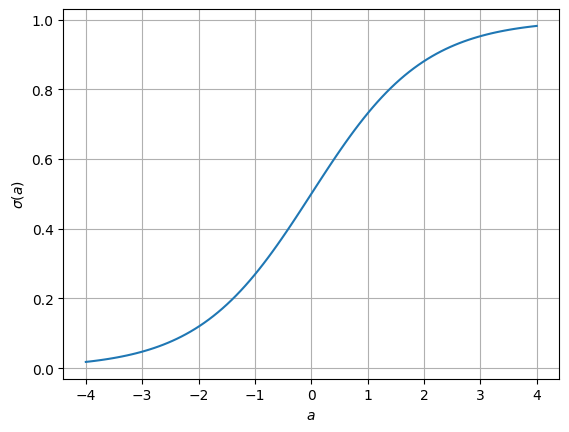
\includegraphics[width=0.6\textwidth]{03_logreg/output_6_0.png}
    \end{center}
\end{frame}

\begin{frame}[allowframebreaks]{Nice Properties of the Logistic Function}\label{logistic-regression}
    \begin{itemize}
        \item Monotonically increasing
        \item Invertible: \(\mbbeta^\top \mbx\) correspond to the \textbf{log odds} of the binary response since the inverse of the sigmoid function is the \textbf{logit function}, 
        \begin{align*}
        \mbbeta^\top \mbx = \sigma^{-1}(\pi(\mbx)) &= \log \frac{\pi(\mbx)}{1 - \pi(\mbx)}.
        \end{align*}

        \item Simplifies some calculations for MLE
    \end{itemize}

Another common mean function is the Gaussian CDF, and we'll consider
that in a later chapter.
\end{frame}

\begin{frame}[t,allowframebreaks]{Hacky Parameter Estimation with
OLS}\label{hacky-parameter-estimation-with-ols}

How do we estimate the parameters, \(\hat{\mbbeta}\)?

If the model were linear, then our first inclination might be to use ordinary least
squares (OLS). Of course, the sigmoidal function above renders the model
nonlinear.

\textbf{Idea:} What if we just used a Taylor approximation around the
origin, 
\begin{align*}
\sigma(a) &\approx \sigma(0) + \sigma'(0) a 
= \frac{1}{2} + \frac{a}{4}
\end{align*}
\end{frame}

\begin{frame}[allowframebreaks]{Hacky Parameter Estimation with OLS}

\begin{center}
    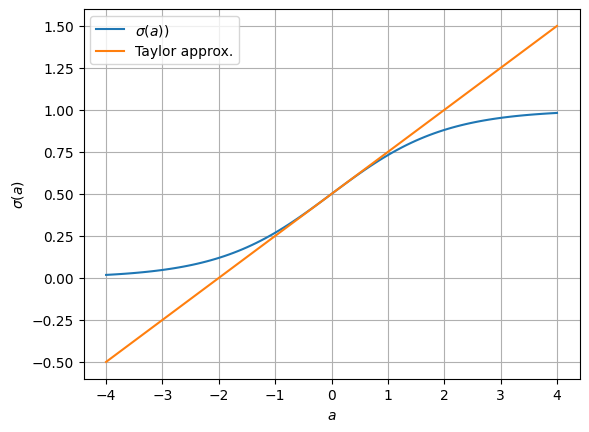
\includegraphics[width=0.6\textwidth]{03_logreg/output_10_0.png}
\end{center}
\end{frame}

\begin{frame}[t,allowframebreaks]{Hacky Parameter Estimation with OLS}
Then under this model, \begin{align*}
\E[Y \mid \mbX=\mbx] 
&\approx \frac{1}{2} + \frac{\mbbeta^\top \mbx}{4} 
\end{align*} or equivalently, \begin{align*}
\E[Z \mid \mbX=\mbx] 
&\approx \mbbeta^\top \mbx
\end{align*} where \(Z = 4 (Y - \tfrac{1}{2}) \in \{-2, +2\}\) is an
adjusted response variable.

Given a set of \(n\) observations of features and (adjusted) responses,
\(\{\mbx_i, z_i\}_{i=1}^n\), the OLS estimate is, \begin{align*}
\hat{\mbbeta}_{\textsf{OLS}} &= \left( \sum_{i=1}^n \mbx_i \mbx_i^\top \right)^{-1} \left(\sum_{i=1}^n \mbx_i z_i \right)
\end{align*}
\end{frame}

\begin{frame}[t,allowframebreaks]{Demo}\label{demo}

Simulated dataset with scalar covariates
\(X_i \sim \mathrm{N}(0,1)\) and responses
\(Y_i \mid X_i = x_i \sim \mathrm{Bern}(\sigma(\beta^* x_i))\) for \(\beta^*=1\).


\begin{center}
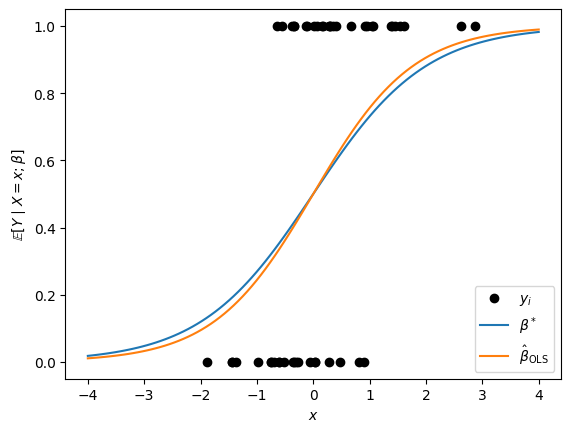
\includegraphics[width=0.5\textwidth]{03_logreg/output_14_1.png}
\end{center}
{ \hspace*{\fill} \\}
    
Not too shabby! Let's try it with a bunch of simulated datasets.
        
\begin{center}
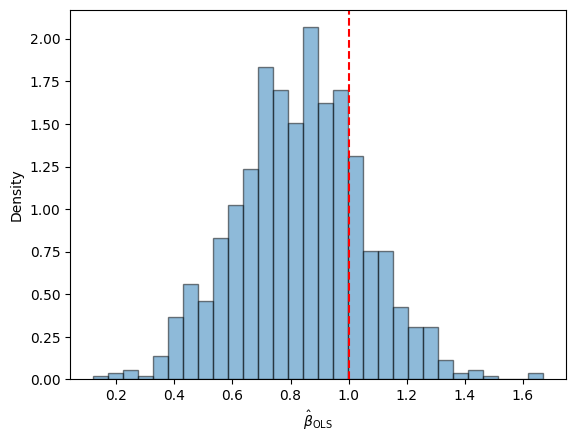
\includegraphics[width=0.5\textwidth]{03_logreg/output_16_1.png}
\end{center}
{ \hspace*{\fill} \\}
    
It looks a bit biased, but it's not terrible.

What if we try for other values of \(\beta^*\)?
\begin{center}
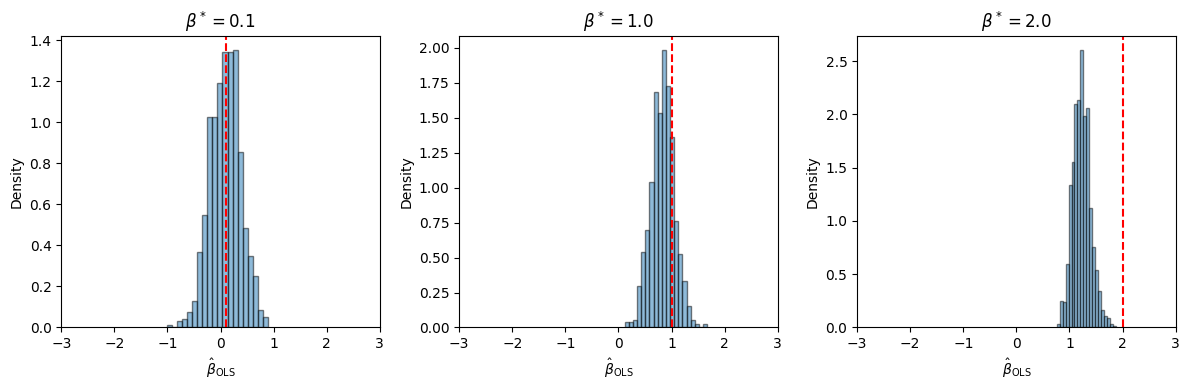
\includegraphics[width=0.8\textwidth]{03_logreg/output_18_0.png}
\end{center}
{ \hspace*{\fill} \\}



\textbf{Question:} Why do you think the OLS estimator becomes more biased as \(\beta^*\)
grows?

\end{frame}

\begin{frame}[t,allowframebreaks]{Maximum Likelihood
Estimation}\label{maximum-likelihood-estimation}

For
standard linear regression with independent Gaussian responses and
homoskedastic noise,
\(\hat{\mbbeta}_{\mathsf{MLE}} = \hat{\mbbeta}_{\mathsf{OLS}}\).

Unfortunately, for logistic regression, there isn't a closed form for
\(\hat{\mbbeta}_{\mathsf{MLE}}\). However, we can use standard
optimization techniques to compute it.

There are plenty of standard implementations of maximum likelihood
estimation for logistic regression models. Let's see how scikit-learn's
implementation fares on the simulated datasets above.
\end{frame}

\begin{frame}[allowframebreaks]{Demo}\label{demo}

\begin{center}
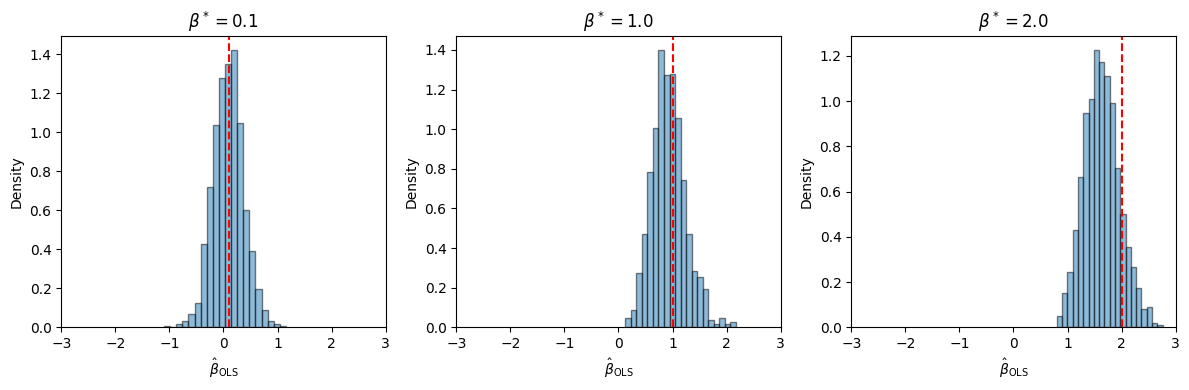
\includegraphics[width=0.8\textwidth]{03_logreg/output_23_0.png}
\end{center}
{ \hspace*{\fill} \\}

\end{frame}

\begin{frame}[t,allowframebreaks]{Deriving the MLE}\label{deriving-the-mle}

Maximizing the likelihood is equivalent to minimizing the (average)
negative log likelihood for a collection of covariates and responses,
\(\{\mbx_i, y_i\}_{i=1}^n\), \begin{align*}
\cL(\mbbeta) 
&= - \frac{1}{n} \sum_{i=1}^n \log \mathrm{Bern}(y_i; \pi(\mbx_i)) \\
&= - \frac{1}{n} \sum_{i=1}^n y_i \log \pi(\mbx_i) + (1 - y_i) \log (1 - \pi(\mbx_i)) \\
&= - \frac{1}{n} \sum_{i=1}^n y_i \log \frac{\pi(\mbx_i)}{1 - \pi(\mbx_i)} + \log (1 - \pi(\mbx_i)) \\
&= - \frac{1}{n} \sum_{i=1}^n y_i \mbbeta^\top \mbx_i + \log (1 - \pi(\mbx_i)).
\end{align*} 
Since $\mbbeta^\top \mbx_i$ is the log odds, as shown above.

Plugging in the definition of $\pi(\mbx_i)$, the second term simplifies as well,
\begin{align*}
\cL(\mbbeta) 
&= - \frac{1}{n} \sum_{i=1}^n \left[y_i \mbbeta^\top \mbx_i + \log \left(1 - \frac{e^{\mbbeta^\top \mbx_i}}{1 + e^{\mbbeta^\top \mbx_i}} \right) \right] \\
&= - \frac{1}{n} \sum_{i=1}^n \left[y_i \mbbeta^\top \mbx_i - \log \left(1 + e^{\mbbeta^\top \mbx_i} \right) \right].
\end{align*}
\end{frame}

\begin{frame}[t,allowframebreaks]{Computing the Gradient}\label{computing-the-gradient}

To minimize the negative log likelihood, take the gradient,
\begin{align*}
\nabla \cL(\mbbeta) 
&= -\frac{1}{n} \sum_{i=1}^n \left(y_i \mbx_i - \frac{e^{\mbbeta^\top \mbx_i}}{1 + e^{\mbbeta^\top \mbx_i}} \mbx_i \right) \\
&= -\frac{1}{n}  \sum_{i=1}^n \left(y_i - \sigma(\mbbeta^\top \mbx_i) \right) \mbx_i.
\end{align*} 

The gradient is a weighted sum of the covariates, and
the weights are the residuals \(y_i - \sigma(\mbx_i^\top \mbbeta)\),
i.e., the difference between the observed and expected response.

\textbf{Intuition:}  move in the direction of covariates where the residual
is positive (we are underestimating the mean), and opposite covariates where the residual is negative
(where we are overestimating the mean).

\textbf{Algorithm:}
\begin{align*}
\mbbeta_{t+1} &\leftarrow \mbbeta_t - \alpha_t \nabla \cL(\mbbeta_t),
\end{align*} 
where \(\alpha_t \in \reals_+\) is the step-size at
iteration \(i\) of the algorithm. 

If the step sizes are chosen
appropriately and the objective is well behaved, the alorithm converges
to at least a local optimum of the log likelihood.
\end{frame}

\begin{frame}[t,allowframebreaks]{Convexity of the Log
Likelhood}\label{convexity-of-the-log-likelhood}

If the objective is convex, then all local optima are also global
optima, and we can give stronger guarantees on gradient descent. To
check the convexity of the log likelihood, we need to compute its
Hessian, \begin{align*}
\nabla^2 \cL(\mbbeta) 
&= \frac{1}{n} \sum_{i=1}^n \sigma'(\mbbeta^\top \mbx_i) \mbx_i \mbx_i^\top
\end{align*} where \(\sigma'(a)\) is the derivative of the logistic
function. That is, \begin{align*}
\sigma'(a) 
&= \frac{\dif}{\dif a}  \sigma(a)\\
&= \frac{e^a}{(1+e^a)^2} \\
&= \sigma(a) (1 - \sigma(a)).
\end{align*} Plugging this in, \begin{align*}
\nabla^2 \cL(\mbbeta) 
&= \frac{1}{n} \sum_{i=1}^n \sigma(\mbbeta^\top \mbx_i)(1 - \sigma(\mbbeta^\top \mbx_i)) \mbx_i \mbx_i^\top \\
&= \frac{1}{n} \sum_{i=1}^n w_i \mbx_i \mbx_i^\top,
\end{align*} where the weights are,
\(w_i = \sigma(\mbbeta^\top \mbx_i)(1 - \sigma(\mbbeta^\top \mbx_i)) = \Var[Y \mid \mbX = \mbx_i]\).


The Hessian is a weighted sum of outer products of
covariates where the weights are equal to the conditional variance, which are non-negative.

Since $w_i > 0$, the Hessian is \textbf{positive semi-definite}, which implies that the
negative log likelihood is convex.
\end{frame}

\begin{frame}[t,allowframebreaks]{Example}\label{example}

As an example, let's plot the negative log likelihood for a scalar
covariate example, as above.
\begin{center}
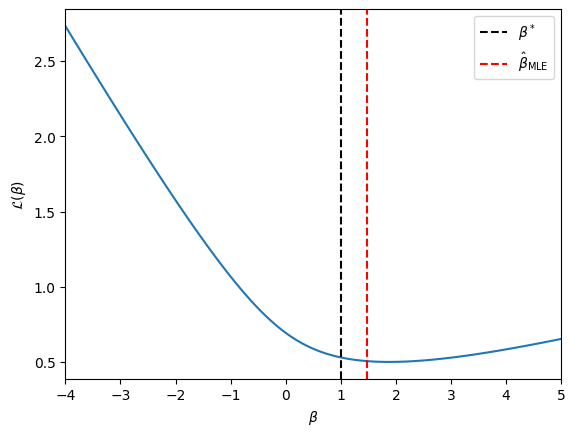
\includegraphics[width=0.5\textwidth]{03_logreg/output_29_0.png}
\end{center}
\end{frame}


\begin{frame}[t,allowframebreaks]{Pathologies in the Separable
Regime}\label{pathologies-in-the-separable-regime}

Suppose the two classes are \emph{linearly separable}, \begin{align*}
\exists \mbu \in \bbS_{p-1} \text{ s.t. } 
\begin{cases}
\mbu^\top \mbx_i > 0 & \text{ if } y_i = 1 \\
\mbu^\top \mbx_i < 0 &\text{ if } y_i = 0
\end{cases}
\end{align*} Now let \(\mbbeta = c \mbu\) for any \(c \in \reals_+\). We
have \begin{align*}
\lim_{c \to \infty} \sigma(c \mbu^\top \mbx_i) &= y_i.
\end{align*} In this limit, the model is saturated:
\(\Pr(y_i \mid \mbx_i) = 1\) for all \(i=1,\ldots,n\); the negative log
likelihood goes to \(\lim_{c \to \infty} \cL(c \mbu) = 0\); and the MLE
does not exist since \(\mbbeta^\star\) diverges.

If we run gradient descent in this setting, the magnitude of the
estimate \(\hat{\mbbeta}\) will grow without bound, while the objective
converges to zero. 
\end{frame}

\begin{frame}[t,allowframebreaks]{\texorpdfstring{\(L_2\)-Regularization}{L\_2-Regularization}}\label{l_2-regularization}

These pathologies can be averted with a little regularization,
\begin{align*}
\cL(\mbbeta) 
&= - \frac{1}{n} \sum_{i=1}^n \log \mathrm{Bern}(y_i; \sigma(\mbbeta^\top \mbx_i)) + \textcolor{red}{\frac{\gamma}{2} \|\mbbeta\|_2^2}.
\end{align*} The regularizer penalizes larger values of the weights,
\(\mbbeta\), and the \textbf{hyperparameter} \(\gamma \in \reals_+\)
sets the strength of the penalty. Even in the linearly separable regime,
the maximizer is finite.

Now, the gradient and Hessian are, \begin{align*}
\nabla \cL(\mbbeta) 
&= -\frac{1}{n}  \sum_{i=1}^n \left(y_i - \sigma(\mbx_i^\top \mbbeta) \right) \mbx_i \textcolor{red}{+ \gamma \mbbeta} \\
\nabla^2 \cL(\mbbeta) 
&= \frac{1}{n} \sum_{i=1}^n w_i \mbx_i \mbx_i^\top \textcolor{red}{+ \gamma \mbI}. 
\end{align*}
\end{frame}

\begin{frame}[t,allowframebreaks]{Choosing the
Hyperparameter}\label{choosing-the-hyperparameter}

There are many ways to select a value of \(\gamma\). 

One approach is to \emph{not} choose a single value and instead try
to compute the \textbf{regularization path}; i.e., the solution
\(\hat{\mbbeta}(\gamma)\) for a range of \(\gamma \in [0, \infty)\).

Another is to hold out a fraction of data and use cross-validation to
select the hyperparameter setting that yields the best performance on
the held-out data.
\end{frame}

\begin{frame}[t,allowframebreaks]{Bayesian Perspective}\label{bayesian-perspective}

From a Bayesian perspective, we can think of the regularizer as a
\textbf{prior log probability}. 

Here, the regularizer corresponds to a spherical Gaussian prior, 
\begin{align*}
\mbbeta &\sim \mathrm{N}(\mbzero, (\gamma n)^{-1} \mbI),
\end{align*} where \textbf{precision (inverse covariance)}
\(\gamma n \mbI\). 

Minimizing the objective above corresponds to doing
\textbf{maximum a posteriori (MAP)} estimation in the Bayesian model. 

We'll talk more about Bayesian methods in the coming weeks.
\end{frame}

\begin{frame}[t,allowframebreaks]{Newton's Method}\label{newtons-method}

Gradient descent leverages the gradient at \(\mbbeta\) to determine the
update. Newton's method uses the Hessian to inform the update as well,
and in doing so it can achieve considerably faster convergence.

The second order Taylor approximation of \(\cL\) around \(\mbbeta\) is
\begin{align*}
\cL(\mbbeta') \approx \cL(\mbbeta) + \nabla \cL(\mbbeta)^\top (\mbbeta' - \mbbeta) + \frac{1}{2} (\mbbeta' - \mbbeta)^\top \nabla^2 \cL(\mbbeta) (\mbbeta' - \mbbeta) \triangleq \widetilde{\cL}(\mbbeta')
\end{align*} 

The stationary point of \(\widetilde{\cL}(\mbbeta')\) is at
\begin{align*}
\nabla \widetilde{\cL}(\mbbeta') &= \nabla \cL(\mbbeta) + \nabla^2 \cL(\mbbeta) (\mbbeta' - \mbbeta) = 0 \\
\implies \mbbeta' &= \mbbeta - [\nabla^2 \cL(\mbbeta)]^{-1} \nabla \cL(\mbbeta),
\end{align*} 
assuming the Hessian is invertible. When
\(\nabla^2 \cL(\mbbeta) \succ 0\) --- i.e., when the Hessian is positive
definite --- the inverse Hessian exists and the stationary point is a
minimizer.

Vanilla Newton's method applies this update repeatedly until
convergence, forming a quadratic approximation and then minimizing it.

\emph{Damped} Newton's method adds a step size \(\alpha_t < 1\) to
improve stability, \begin{align*}
\mbbeta_{t+1} &\leftarrow \mbbeta_t - \alpha_t [\nabla^2 \cL(\mbbeta_t)]^{-1} \nabla \cL(\mbbeta_t),
\end{align*} 
The step size can be chosen by backtracking line
search.

\textbf{Question:} Compare the Newton update to that of gradient
descent. How do they differ?

\end{frame}

\begin{frame}[t,allowframebreaks]{Iteratively Reweighted Least
Squares}\label{iteratively-reweighted-least-squares}

% Newton's method solves for the minimum of a quadratic approximation to
% the loss function at each iteration. What else involves minimizing a
% quadratic loss function? Least squares! 

Newton's method can be viewed as iteratively solving a weighted least squares
problem. 

Write the gradient and Hessian in matrix form, \begin{align*}
\nabla \cL(\mbbeta_t) &= -\frac{1}{n} \mbX^\top (\mby - \hat{\mby}_t) \\
\nabla^2 \cL(\mbbeta_t) &= \frac{1}{n} \mbX^\top \mbW_t \mbX
\end{align*} 
where 
\begin{itemize}
    \item \(\mbX \in \reals^{n \times p}\) is the design
matrix with rows \(\mbx_i^\top\) 
    \item \(\mby \in \{0,1\}^n\) is the vector
of binary responses 
    \item \(\hat{\mby}_t = \sigma(\mbX \mbbeta_t) \in [0,1]^n\) is the vector of
predicted response means 
    \item \(\mbW_t = \diag([w_{t,1}, \ldots, w_{t,n}])\) with
\(w_{t,i} = \sigma(\mbx_i^\top \mbbeta_t) (1- \sigma(\mbx_i^\top \mbbeta_t))\)
is the diagonal weight matrix.
\end{itemize}

Then the (undamped) Newton update is, \begin{align*}
\mbbeta_{t+1} 
&= \mbbeta_t - [\nabla^2 \cL(\mbbeta_t)]^{-1} \nabla \cL(\mbbeta_t) \\
&= \mbbeta_t + [\mbX^\top \mbW_t \mbX]^{-1} \mbX^\top (\mby - \hat{\mby}_t) \\
&= [\mbX^\top \mbW_t \mbX]^{-1} \mbX^\top \mbW_t \mbX \mbbeta_t + [\mbX^\top \mbW_t \mbX]^{-1} \mbX^\top (\mby - \hat{\mby}_t) \\
&= [\mbX^\top \mbW_t \mbX]^{-1} \mbX^\top \mbW_t \mbz_t
\end{align*} 
where 
\begin{align*}
\mbz_t &= \mbX \mbbeta_t + \mbW_t^{-1} (\mby - \hat{\mby}_t).
\end{align*} 

This is a \textbf{weighted least squares} problem with \textbf{weights}
\(w_{t,i}\) and \textbf{adjusted (or working) responses} \(z_{t,i}\).

How can we interpret the working responses? We can view them as the real
responses mapped through a Taylor approximation of the link (inverse
mean) function, 
\begin{align*}
\sigma^{-1}(y_i) 
&\approx \sigma^{-1}(\hat{y}_{t,i}) + (y_i - \hat{y}_{t,i}) [\sigma^{-1}]'(\hat{y}_{t,i}) \\
&= \mbx_i^\top \mbbeta_t + \frac{(y_i - \hat{y}_{t,i})}{w_{t,i}} \\
&\triangleq z_{t,i}.
\end{align*}
\end{frame}

\begin{frame}[t,allowframebreaks]{Asymptotic Covariance of
MLE}\label{asymptotic-covariance-of-mle}

What other insight can we glean from the Hessian? Recall our discussion
of the asymptotic normality of the MLE from
\href{01_distributions.ipynb}{Lecture 1}. For iid observations
\(Y_i \iid{\sim} p(\cdot; \mbtheta)\) for \(i=1,\ldots,n\), the
asymptotic covariance is \(\cI(\mbtheta)^{-1} / n\), where
\begin{align*}
\cI(\mbtheta)= -\E[\nabla_{\mbtheta}^2 \log p(Y; \mbtheta)]
\end{align*} is the Fisher information matrix.

For logistic regression, we have \(n\) independent but \emph{not}
identically distributed observations. In this case, the asymptotic
covariance follows the same form. It is given by the inverse of the
Fisher information matrix; i.e., the inverse of the negative expected
Hessian of the log likelihood, \begin{align*}
\cI(\mbbeta) = -\sum_{i=1}^N \E[\nabla_{\mbbeta}^2 \log p(Y_i \mid \mbX_i=\mbx_i; \mbbeta)].
\end{align*} (Note that this includes the iid formula as a special
case.)

Substituting the form of the Hessian from above, \begin{align*}
\cI(\mbbeta)
&= \sum_{i=1}^n \E[\Var[Y_i \mid \mbX = \mbx_i] \mbx_i \mbx_i^\top] \\
&= \sum_{i=1}^n w_i \mbx_i \mbx_i^\top 
\end{align*} where
\(w_i = \sigma(\mbbeta^\top \mbx_i) (1 - \sigma(\mbbeta^\top \mbx_i))\).
Finally, we evaluate the Fisher information the MLE to obtain the
asymptotic covariance estimate, \begin{align*}
\widehat{\Cov}(\hat{\mbbeta}) &= [\cI(\hat{\mbbeta})]^{-1}.
\end{align*}

Like before, we can use the asymptotic covariance estimate to derive
Wald confidence intervals for the parameters and perform hypothesis
tests.

\textbf{Caution:} Remember, Wald confidence
intervals are only as good as the asymptotic normality assumption. When
the likelihod is not well approximated by a quadratic, the covariance
estimate will be poor, and the confidence intervals will be invalid.
When might the Gaussian approximation not hold? :::
\end{frame}


\begin{frame}[t,allowframebreaks]{Converge Rate of Gradient
Descent}\label{converge-rate-of-gradient-descent}

To determine when and at what rate gradient descent converges, we need
to know more about the eigenvalues of the Hessian.

If we can bound the maximum eigenvalue of the Hessian by \(L\), then we
can obtain a quadratic upper bound on the negative log likelihood,
\begin{align*}
\cL(\mbbeta') &\leq \cL(\mbbeta) + \nabla \cL(\mbbeta)^\top (\mbbeta' - \mbbeta) + \frac{L}{2} (\mbbeta' - \mbbeta)^\top (\mbbeta' - \mbbeta).
\end{align*} That means the negative log likelihood is an \(L\)-smooth
function.
\end{frame}

\begin{frame}[t,allowframebreaks]{Converge Rate of Gradient
    Descent}\label{converge-rate-of-gradient-descent}
\textbf{Example:} Bounded Covariates

If the covariates have bounded norm, \(\|\mbx_i\|_2 \leq B\), then we
can bound the maximum eigenvalue of the Hessian by, \begin{align*}
\lambda_{\mathsf{max}} 
&= \max_{\mbu \in \bbS_{p-1}} \mbu^\top \nabla^2 \cL(\mbbeta) \mbu \\
&= \max_{\mbu \in \bbS_{p-1}} \frac{1}{n} \sum_{i=1}^n w_i \mbu^\top \mbx_i \mbx_i^\top \mbu \\
&\leq \frac{B^2}{4}
\end{align*} since the weights are the conditional variances of
Bernoulli random variables, which are at most \(\tfrac{1}{4}\), and
since \(\mbu^\top \mbx_i \leq B\) for all unit vectors
\(\mbu \in \bbS_{p-1}\) (the unit sphere embedded in \(\reals^p\)). This
isn't meant to be a tight upper bound. 
% End of example

If we run gradient descent with a constant step size of
\(\alpha = 1/L\), then the algorithm converges at a rate of \(1/t\),
which means that after \(t\) iterations \begin{align*}
\cL(\mbbeta^\star) - \cL(\mbbeta_t) \leq \frac{L}{t} \|\mbbeta^\star - \mbbeta_0\|_2^2,
\end{align*} where \(\mbbeta_0\) is the initial setting of the
parameters and \(\mbbeta^\star\) is the global optimum.

Put differently, if we want a gap of at most epsilon, we need to run
\(t \sim \cO(1/\epsilon)\) iterations of gradient descent. Put
differently, if we want to reduce \(\epsilon\) by a factor of 100, we
need to run around 100 times as many iterations. This is called a
\textbf{sub-linear convergence} rate.
\end{frame}

\begin{frame}[t,allowframebreaks]{Converge Rate of Gradient Descent with
Regularization}\label{converge-rate-of-gradient-descent-with-regularization}

With regularization, we can also \textbf{lower bound} the objective by a
quadratic function, \begin{align*}
\cL(\mbbeta') &\geq \cL(\mbbeta) + \nabla \cL(\mbbeta)^\top (\mbbeta' - \mbbeta) + \frac{\mu}{2} (\mbbeta' - \mbbeta)^\top (\mbbeta' - \mbbeta)
\end{align*} for \(\mu > 0\), which means the objective is
\(\mu\)-\textbf{strongly convex}.

For twice differentiable objectives, the minimum eigenvalue of Hessian
provides such a lower bound, \(\mu = \lambda_{\mathsf{min}}\). In
particular, we know that minimum eigenvalue of \(\nabla^2 \cL(\mbbeta)\)
is at least \(\gamma\). (This bound is achieved when the data are
linearly separable, the model is saturated, and the conditional
variances are all zero.)

For a \(L\)-smooth and \(\mu\)-strongly convex function with stepsize
\(\alpha = 1/L\), gradient descent has the following convergence
guarantee, \begin{align*}
\cL(\mbbeta_{t+1}) - \cL(\mbbeta^\star) &\leq \left(1 - \frac{\mu}{L} \right) (\cL(\mbbeta_t) - \cL(\mbbeta^\star)).
\end{align*} Applying this bound recursively yields that, \begin{align*}
\cL(\mbbeta_t) - \cL(\mbbeta^\star) &\leq \left(1 - \frac{\mu}{L} \right)^t (\cL(\mbbeta_0) - \cL(\mbbeta^\star)).
\end{align*} If we want to find the number of iterations \(t\) to bound
the gap by at most \(\epsilon\), we need to solve for \(t\) in
\begin{align*}
\left(1 - \frac{\mu}{L}\right)^t ( \mathcal L(\beta_0) - \mathcal L(\beta^*)) \leq \epsilon.
\end{align*} This inequality is equivalent to taking the log of both
sides \begin{align*}
    \log ( \mathcal L(\beta_0) - \mathcal L(\beta^*)) + t \log\left(1 - \frac{\mu}{L}\right) \leq \log \epsilon.
\end{align*} We can further upper bound the LHS by using the inequality
\(\log ( 1 - x) \leq -x\) to get \begin{align}
    \log ( \mathcal L(\beta_0) - \mathcal L(\beta^*))  - \frac{\mu t}{L}\leq \log \epsilon.
\end{align} So, we need to run
\(t \geq \frac{L}{\mu} \log \frac{\cL(\mbbeta_0) - \cL(\mbbeta^\star)}{\epsilon} \sim \log \frac{1}{\epsilon}\)
iterations of gradient descent. If we want to reduce \(\epsilon\) by a
factor of 100, we only need to run around \(\log 100\) times as many
iterations. This is called \textbf{linear convergence}.
\end{frame}

\begin{frame}[t,allowframebreaks]{Converge Rate of Newton's
Method}\label{converge-rate-of-newtons-method}

Under certain conditions --- if the objective is strongly convex, the
Hessian is Lipschitz continuous, and we start near enough to the global
optimum --- Newton's method achieves \textbf{second order convergence},
meaning \begin{align*}
\|\mbbeta_{t+1} - \mbbeta^\star\|_2 \leq \left(c \|\mbbeta_t - \mbbeta^\star\|_2\right)^2
\end{align*} for some positive constant \(c\), provided we start with
\(\mbbeta_0\) close enough to \(\mbbeta^\star\). Applying this bound
recursively yields that, \begin{align*}
\|\mbbeta_t - \mbbeta^\star\|_2 &\leq \left(c \|\mbbeta_0 - \mbbeta^\star\|_2 \right)^{2^t}.
\end{align*}

Put differently, if we start with
\(\|\mbbeta_0 - \mbbeta^\star\| < c^{-1}\), then we need
\(t \sim \cO(\log \log \frac{1}{\epsilon})\) iterations to obtain an
error of \(\epsilon\). Since the double log grows incredibly slowly,
this statement says that we effectively need a constant number of
iterations for Newton's method to converge in this regime.

For more information on convergence rates of gradient descent and
Newton's method, see \{cite:t\}\texttt{boyd2004convex}, ch.~9.
\end{frame}

\begin{frame}[t,allowframebreaks]{Conclusion}\label{conclusion}

One, two, many\ldots{} with logistic regression, we can begin modeling
relationships between binary response variables and (possibly
arbitrary-valued) covariates. Next, we'll see how to expand from
logistic regression to generalized linear models for exponential family
responses.
\end{frame}

\end{document}
